\documentclass[3p, authoryear]{elsarticle} %review=doublespace preprint=single 5p=2 column
%%% Begin My package additions %%%%%%%%%%%%%%%%%%%
\usepackage[hyphens]{url}

  \journal{Submitted to Journal} % Sets Journal name


\usepackage{lineno} % add
\providecommand{\tightlist}{%
  \setlength{\itemsep}{0pt}\setlength{\parskip}{0pt}}

\usepackage{graphicx}
\usepackage{booktabs} % book-quality tables
%%%%%%%%%%%%%%%% end my additions to header

\usepackage[T1]{fontenc}
\usepackage{lmodern}
\usepackage{amssymb,amsmath}
\usepackage{ifxetex,ifluatex}
\usepackage{fixltx2e} % provides \textsubscript
% use upquote if available, for straight quotes in verbatim environments
\IfFileExists{upquote.sty}{\usepackage{upquote}}{}
\ifnum 0\ifxetex 1\fi\ifluatex 1\fi=0 % if pdftex
  \usepackage[utf8]{inputenc}
\else % if luatex or xelatex
  \usepackage{fontspec}
  \ifxetex
    \usepackage{xltxtra,xunicode}
  \fi
  \defaultfontfeatures{Mapping=tex-text,Scale=MatchLowercase}
  \newcommand{\euro}{€}
\fi
% use microtype if available
\IfFileExists{microtype.sty}{\usepackage{microtype}}{}
\usepackage{natbib}
\bibliographystyle{apalike}
\usepackage{longtable}
\usepackage{graphicx}
\ifxetex
  \usepackage[setpagesize=false, % page size defined by xetex
              unicode=false, % unicode breaks when used with xetex
              xetex]{hyperref}
\else
  \usepackage[unicode=true]{hyperref}
\fi
\hypersetup{breaklinks=true,
            bookmarks=true,
            pdfauthor={},
            pdftitle={Examining the Utility-based Resiliency of Utah's Highway Network},
            colorlinks=false,
            urlcolor=blue,
            linkcolor=magenta,
            pdfborder={0 0 0}}
\urlstyle{same}  % don't use monospace font for urls

\setcounter{secnumdepth}{5}
% Pandoc toggle for numbering sections (defaults to be off)

% Pandoc citation processing

% Pandoc header
\usepackage{booktabs}
\usepackage{booktabs}
\usepackage{longtable}
\usepackage{array}
\usepackage{multirow}
\usepackage{wrapfig}
\usepackage{float}
\usepackage{colortbl}
\usepackage{pdflscape}
\usepackage{tabu}
\usepackage{threeparttable}
\usepackage{threeparttablex}
\usepackage[normalem]{ulem}
\usepackage{makecell}
\usepackage{xcolor}



\begin{document}
\begin{frontmatter}

  \title{Examining the Utility-based Resiliency of Utah's Highway Network}
    \author[Brigham Young University]{Gregory Macfarlane}
   \ead{gregmacfarlane@byu.edu} 
    \author[Brigham Young University]{Max Barnes}
   \ead{barnesmaxmax@gmail.com} 
    \author[Brigham Young University]{Natalie Gray}
   \ead{nat.gray2000@gmail.com} 
      \address[Brigham Young University]{Brigham Young University, Civil and Environmental Engineering Department, 430 Engineering Building, Provo, Utah 84602}
      \cortext[1]{Corresponding Author}
  
  \begin{abstract}
  This is where the abstract should go.
  \end{abstract}
   \begin{keyword} Accessibility Passive Data Location Choice\end{keyword}
 \end{frontmatter}

\hypertarget{intro}{%
\section{Introduction}\label{intro}}

Systemic resiliency is an important consideration for transportation agencies,
though specific definitions of ``resiliency'' might vary under different contexts.
Some agencies and researchers see resiliency as facility-level design and
engineering that hardens the system against failure \citep{bradley2007, peeta2010};
others as an ability for maintenance staff to rapidly restore service following
catastrophe \citep{zhang2016}; and others as an ability for a system to continue
operating in degraded state \citep{berdica2002, ip2011}. Regardless of the
definition used, assessing the resiliency of a transportation network --- and
addressing any potential shortfalls --- requires a method to identify which
links or facilities are most critical to the smooth operation of the network.

Identifying which links in a transportation network are most critical, however,
is not trivial. State of the practice techniques typically rely on traffic volumes
represented in terms of vehicles, trips, or freight value \citep{aem2017}. But these
methods ignore the fact that some networks have alternate routes readily available,
have multiple well developed modes of transportation, or have redundant
destination locations. When a network link does break, routes, mode choice, and
destination choice often change too. These responses have been observed in
real-world crisis events like the I-35 W bridge collapse in Minneapolis and the
I-85 bridge fire and collapse in Atlanta
\citep{zhu2010, levinson2010, xie2011, hamedi2018}.

In this research, we apply destination choice accessibility model to identify
critical highway links in a statewide highway context. This model is designed to
capture the utility lost to individuals operating on a degraded network who may
choose a longer route, a different travel mode, or a different destination. We
then apply the model to a highway network representing the state of Utah. The
model structure permits a more nuanced evaluation of link criticality than using
traffic volume alone or in conjunction with an increased travel time measure.

The paper proceeds as follows. First, a \protect\hyperlink{litreview}{literature review} discusses
previous attempts to analyze the resiliency of transportation networks. A
\protect\hyperlink{methodology}{methodology} section presents the model developed for this
research and describes the implementation process in Utah. A \protect\hyperlink{results}{results} section
describes the model output in detail for one scenario and then compares and ranks
the model outputs for an array of several dozen independent scenarios. The paper
\protect\hyperlink{conclusion}{concludes} with a discussion of limitations and associated avenues
for future research.

\hypertarget{litreview}{%
\section{Literature}\label{litreview}}

In a groundbreaking theoretical article, \citet{berdica2002} attempted to identify,
define and conceptualize network ``vulnerability'' --- the complement of
resiliency --- by envisioning analyses conducted with
several vulnerability performance measures including travel time, delay,
congestion, serviceability, and accessibility. She then defined reliability as
the level of reduced accessibility due to unfavorable operating conditions on
the network. In particular, Berdica identified a need for further research
toward developing a framework capable of investigating reliability of
transportation networks.

In this section we examine several attempts by numerous researchers to do
precisely this using various measures of network performance. It is helpful to
categorize this review into three groups based on the overall technique applied
in the study:

\begin{itemize}
\item
  \emph{Network connectivity}: How does damage to a network diminish the connectivity
  between network nodes?
\item
  \emph{Travel time analysis}: How much do shortest path travel times between origins
  and destinations increase on a damaged network?
\item
  \emph{Accessibility analysis} How easily can the population using the damaged
  network complete their daily activities?
\end{itemize}

The following sections discuss relevant studies in each group; Table
\ref{tab:authortable} consolidates these studies by year and labels them with
an applicable group.

\begin{table}

\caption{\label{tab:authortable}Attempts to Evaluate Systemic Resiliency}
\centering
\begin{tabular}[t]{rll}
\toprule
Year & Author & Performance Metric\\
\midrule
2004 & Geurs and van Wee & Accessibility (isochrone, gravity, logsum)\\
2007 & Abdel-Rahim et al. & Network Connectivity\\
2008 & Taylor, M & Accessibility (logsum)\\
2010 & Peeta et al. & Travel time and cost\\
2010 & Geurs et al. & Accessibility (logsum)\\
\addlinespace
2010 & Levinson and Zhu & Travel time and cost\\
2010 & Zhu et al. & Travel time and cost\\
2011 & Agarwal et al. & Network connectivity\\
2011 & Ip and Wang & Network connectivity\\
2011 & Serulle et al. & Travel time and cost\\
\addlinespace
2011 & Ibrahim, S & Travel time and cost\\
2011 & Xie and Levinson & Accessibility (isochrone)\\
2013 & Omer et al. & Travel time and cost\\
2014 & Osei-Asamoah and Lownes & Network connectivity\\
2015 & Zhang et al. & Network connectivity\\
\addlinespace
2015 & Guze & Network connectivity\\
2015 & Jaller et al. & Travel time and cost\\
2015 & Xu et al. & Network connectivity\\
2016 & Winkler, C. & Accessibility (gravity)\\
2017 & Ganin et al. & Accessibility (gravity)\\
\addlinespace
2019 & Vodak et al. & Network connectivity\\
2019 & Hackl and Adey & Network connectivity\\
\bottomrule
\end{tabular}
\end{table}

\hypertarget{network-connectivity}{%
\subsection{Network Connectivity}\label{network-connectivity}}

The purpose of transportation networks is to connect locations to each other;
presumably damage to a network would diminish the network's \emph{connectivity}, or
the number of paths between node pairs. It may even leave nodes or groups of nodes
completely isolated. In studies based on connectivity, researchers typically apply
methods and concepts from graph theory.

\citet{abdel2007} developed a multi-layered graph to examine the resiliency of the traffic
signal control system in Boise, Idaho. The researchers determined which
traffic signals would be isolated by a failure to a particular power substation,
and consequentially the percent of travel paths that would experience diminished
levels of service. The research highlights the degree to which interrelated
infrastructure systems --- power, telecommunications, and transportation ---
depend on each other, though the researchers did not attempt to look at the
connective resiliency of the transportation network directly.

\citet{agarwal2011} present a method to represent a transportation network as a
hierarchical graph that can be analyzed more directly for vulnerabilities. The
authors acknowledge, however, that a maximal failure consideration where a node
is entirely isolated from the network is unlikely in a real-world network with
multiple paths of connectivity.

\citet{ip2011} address this shortcoming through the concept of \emph{friability}, or
the reduction of capacity caused by removing a link or node, in order to
determine criticality of individual links. The methodology relies on the ability
to determine the weighted sum of the resilience of all nodes based on the
weighted average of connectedness with other city nodes in the network. The
authors determine that the recovery of transportability between two cities
largely depends on redundant links between nodes. The authors also comment that
most traffic managers are more concerned with the friability of single links
rather than the friability of multiple links or an entire system.

\citet{vodak2019} develop an approach to identify
critical links in a network by searching for the shortest independent
loops in the network. The algorithm progressively damages one or more links
between iterations to determine if nodes become isolated, or cut off from the
network. If a node becomes easily isolated or has a higher likelihood of
becoming isolated, then there is a higher degree of vulnerability present in the
network. This method can both identify critical links in individual networks, as
well as provide a means to quantitatively compare networks.

All of these graph theoretical approaches tend to break down to some degree on
large, real-world networks where the number of nodes and links numbers in the tens
of thousands, and the degree of connectivity between any arbitrary node pair is
high.

\hypertarget{changes-in-travel-time}{%
\subsection{Changes in Travel Time}\label{changes-in-travel-time}}

Highway system network failures --- in most imaginable cases --- degrade the
shortest or least cost path but typically do not eliminate it entirely. The degree
to which travel time increases when a particular link is damaged could provide an
estimate of the criticality of that link.

\citet{peeta2010} construct a model to efficiently allocate
highway maintenance resources. Each link in the sample network was
assigned a specific failure probability based on resource allocation;
the model evaluated the increase in travel time resulting from a broken
link. A Monte Carlo simulation revealed which allocation plan resulted in the least
network degradation, and thus which links were most critical to the network's
operations.

\citet{ibrahim2011} provide an alternative heuristic approach for determining
vulnerability of infrastructure by estimating the cost of single link failure
based on the increase in shortest path travel time due to increased congestion
levels. The authors propose a hybrid heuristic approach that calculates the
traditional user-equilibrium assignment for finding the first set of costs, and
then fixes those costs for all following iterations to determine the effects of
failure on overall travel time of the system. \citet{omer2013} apply a similar methodology
to a real-life intercity highway network. \citet{jaller2015} extended this methodology
with a static user equilibrium traffic loading step to provide an estimate of
how the next-shortest path changes when congested.

A primary limitation with increased travel time methodologies is that they
ignore the other possible ways a population might adapt its travel to a damaged
network. Some people may choose other modes or destinations, and it is possible
that some previously occurring trips might be canceled entirely.

\hypertarget{changes-in-accessibility}{%
\subsection{Changes in Accessibility}\label{changes-in-accessibility}}

In a travel modeling context, \emph{accessibility} refers to the ease with which
individuals can reach the destinations that matter to them; this is an abstract
idea but one that has been quantified in numerous ways. \citet{dong2006} provide a
helpful framework for understanding various quantitative definitions of
accessibility that we will simplify here. The most elementary definition of
accessibility is whether a destination is within an \emph{isochrone}, or certain
distance. This measure is often represented as a count, e.g., the number of jobs
reachable from a particular location within thirty minutes travel time by a
particular mode. Mathematically,

\begin{equation}
A_i = \sum_{j} X_j I_{ij};  I_{ij} = \begin{cases}  1 \text{ if } d_{ij} \leq D\\ 
0 \text{ if } d_{ij} > D \end{cases}
  \label{eq:isochrone}
\end{equation}

where the accessibility \(A\) at point \(i\) is the sum of the all the
destinations \(X\) at other points \(j\). \(I_{ij}\) is an indicator function equal to
zero if the distance between the points \(d{_ij}\) is less than some asserted
threshold (e.g., thirty minutes of travel time). By relaxing the assumption of a
binary isochrone and instead using the distance directly, we can derive the
so-called gravity model,

\begin{equation}
A_i = \sum_{j} X_j f(d_{ij})
  \label{eq:gravity}
\end{equation}

where the function \(f(d_{ij})\) is often a negative exponential with a calibrated
impedance coefficient. An extension of the gravity model is to use the logsum
term of a multinomial logit destination choice model,

\begin{equation}
A_i = ln\sum_{j} \beta_d(d_{ij}) + X_j\beta
  \label{eq:logsum}
\end{equation}

where the parameters \(\beta\) are estimated from choice surveys or calibrated to
observed data. The logsum term has numerous benefits outlined by \citet{handy1997}
and \citet{geurs2004}; namely, the measure is based in actual choice theory, and
can include multiple destination types and travel times by multiple different
modes.

\citet{taylor2008} applied logsum-derived accessibility analysis to evaluate the
consequences of a tunnel failure in Adelaide, Australia.

\begin{enumerate}
\def\labelenumi{\arabic{enumi}.}
\tightlist
\item
  LOOK LITERATURE THAT TAYLOR CITES
\item
  LOOK AT LITERATURE THAT HAS CITED TAYLOR
\item
  TELL THE STORY OF WHY WHAT WE DID IS WORTHWHILE
\end{enumerate}

BECAUSE THERE IS A GAP! STATEWIDE

\hypertarget{methodology}{%
\section{Methodology}\label{methodology}}

The objective of this study is to evaluate the relative systemic criticality of
highway links on a statewide network using a model sensitive to changes in route
path, destination choice, and mode choice. We first describe the model, and then
its implementation.

\hypertarget{model-design}{%
\subsection{Model Design}\label{model-design}}

The overall model framework is presented in Figure \ref{fig:framework}, and is
designed to capture the utility-based accessibility for a particular origin
zones \(i\) and trip purpose \(m\). The model begins with a travel time skim
procedure, to determine the congested travel time from zone \(i\) to zone \(j\) by
auto as well as the shortest network distance for non motorized modes. The
transit travel time skim is fixed, assuming that transit infrastructure would
not be affected by changes to the highway network. Throughout this section,
lower-cased index variables \(k\) belong to a set of all indices described by the
corresponding capital letter \(K\)

\begin{figure}

{\centering 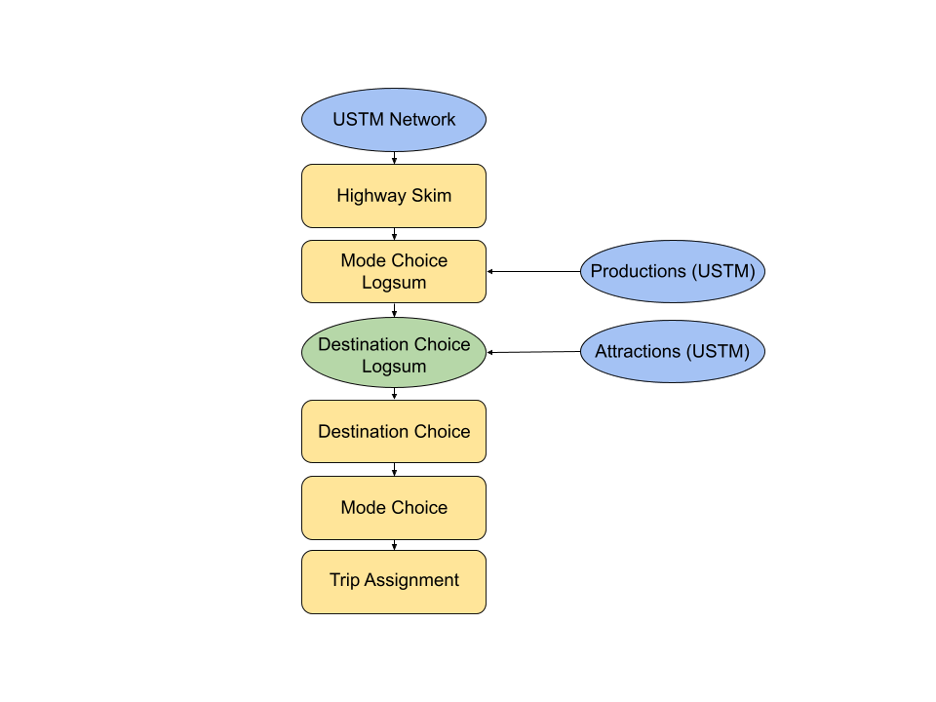
\includegraphics[width=0.75\linewidth]{images/framework} 

}

\caption{Model framework.}\label{fig:framework}
\end{figure}

With the travel time \(t_{ijk}\) for all modes \(k \in K\), the model computes
mode choice utility values. The multinomial logit mode choice model describes
the probability of a person at origin \(i\) choosing mode \(k\) for a trip to
destination \(j\):
\begin{equation}
\mathcal{P}_{ijm}(k) = \frac{\exp(f(\beta_{m}, t_{ijk}))}{\sum_{K}\exp(f(\beta_{m}, t_{ijk}))}
  \label{eq:mcp}
\end{equation}
The log of the denominator of the this equation is called the
mode choice logsum, \(MCLS_{ijm}\) and is a measure of the travel cost by all
modes, weighted by utility parameters \(\beta_m\) that may vary by trip purpose.

The \(MCLS\) is then used as a travel impedance term in the multinomial logit
destination choice model, where the probability of a person at origin \(i\)
choosing destination \(j \in J\) is
\begin{equation}
\mathcal{P}_{im}(j) = \frac{\exp(f(\gamma_{m}, MCLS_{ijm}, A_j))}{\sum_{J}\exp(f(\gamma_{m}, MCLS_{ijm}, A_j))}
  \label{eq:dcp}
\end{equation}
where \(A_j\) is the attractiveness --- represented in terms of socioeconomic activity
--- of zone \(j\). As with mode choice, the log of the denominator of this model is the destination
choice logsum, \(DCLS_{im}\). This quantity represents the value access to all destinations
by all modes of travel, and varies by trip purpose.

The \(DCLS_{im}\) measure is relative, but can be compared across scenarios. The
difference between the measures of two scenarios
\begin{equation}
\Delta_{im} = DCLS_{im}^{\mathrm{Base}} - DCLS_{im}^{\mathrm{Scenario}}
  \label{eq:deltas}
\end{equation}
however, provides an estimate of the accessibility lost when \(t_{ij\mathrm{drive}}\)
changes due to a damaged highway link. This accessibility change is \emph{per trip},
meaning that the total lost accessibility is \(P_{im} * \Delta_{im}\) where \(P\) is
the number of trip productions at zone \(i\) for purpose \(m\). This measure is
given in units of dimensionless utility, but the mode choice cost coefficient
\(\beta\) provides a conversion factor between utility and cost. The total financial
cost of a damaged link for the entire region for all trip purposes is
\begin{equation}
\mathrm{Cost} = \sum_{I}\sum_{M} -1 / \beta_{\mathrm{cost},m} * P_{im} \Delta_{im}
  \label{eq:totalcost}
\end{equation}

For comparison to a simpler resiliency method that only includes the increased
travel time between origins and destinations, we compute the change in travel
time between \(\delta t_{ij}\) and multiply the number of trips by this change
and a value of time coefficient derived from the cost and vehicle time coefficients
of the mode choice model,
\begin{equation}
\mathrm{Cost}' =  \sum_I \sum_J \sum_M \frac{\beta_{\mathrm{time}, m} }{\beta_{\mathrm{cost}, m}} T_{ijm} t_{ijm}
  \label{eq:ttmethod}
\end{equation}

\hypertarget{model-implementation-in-utah}{%
\subsection{Model Implementation in Utah}\label{model-implementation-in-utah}}

The Utah Department of Transportation (UDOT) manages an extensive highway
network consisting of interstate freeways (I-15, I-80, I-70, and I-84),
intraurban expressways along the Wasatch Front, and rural highways throughout
the state. The rugged mountain and canyon topography throughout the state places
severe constraints on possible redundant paths in the highway network. A
landslide or rock fall in any single canyon may isolate a community or force a
redirection of traffic that could be several hours longer than the preferred
route; understanding which of these many choke points is most critical is a key
and ongoing objective of the agency.

Several data elements for the model described above were obtained from the Utah
Statewide Travel Model (USTM). USTM is a trip-based statewide model that is
focused exclusively on long-distance and rural trips: intraurban trips within
existing Metrpolitan Planning Organization (MPO) model regions are pre-loaded
onto the USTM highway network. This means that USTM as currently constituted can
be used for infrastructure planning purposes, but would be inadequate to
evaluate the systemic resiliency of the highway network given the disparate
methodologies of the MPO models. USTM can, however, provide the following
data elements

\begin{enumerate}
\def\labelenumi{\arabic{enumi}.}
\tightlist
\item
  \emph{Highway Network}: including free flow and congested travel speeds,
  link length, link capacity estimates, etc.
\item
  \emph{Zonal Productions} \(P_{im}\): available for all zones by purpose,
  including those in the MPO region areas.
\item
  \emph{Zonal Socioeconomic Data}: the destination choice model described in
  Equation \eqref{eq:dcp} calculates attractions \(A_{jm}\) from the USTM zonal
  socioeconomic data based on the utility coefficients in \ref{tab:coeffs}.
\item
  \emph{Calibration Targets}: USTM base scenario estimates of mode split and
  trip length were used to calibrate the utility coefficients as described
  below.
\end{enumerate}

Among MPO models in Utah, only the model jointly operated by the
Wasatch Front Regional Council (WFRC, Salt Lake area MPO) and the\\
Mountainland Association of Governments (MAG, Provo area MPO) model include a
substantive transit forecasting component. The transit travel time skim from the
WFRC / MAG model was used for the mode choice model in Equation \eqref{eq:mcp};
the zonal travel time between the smaller WFRC / MAG model zones was averaged
to the larger USTM zones, and the minimum time among the several modes available
(commuter rail, light rail, bus rapid transit, local bus) was taken as the travel
time for a single transit mode in this implementation.

\begin{table}

\caption{\label{tab:coeffs}Choice Model Coefficients}
\centering
\begin{tabular}[t]{llrrr}
\toprule
 & Variable & HBW & HBO & NHB\\
\midrule
\addlinespace[0.3em]
\multicolumn{5}{l}{\textbf{Destination Choice}}\\
\hspace{1em} & Households & 0.0000 & 1.0187 & 0.2077\\

\hspace{1em} & Office Employment & 0.4568 & 0.4032 & 0.2816\\

\hspace{1em} & Other Employment & 1.6827 & 0.4032 & 0.2816\\

\hspace{1em} & Retail Employment & 0.6087 & 3.8138 & 5.1186\\

\hspace{1em} & Distance & -0.0801 & -0.1728 & -0.1157\\

\hspace{1em} & Distance\textasciicircum{}2 & 0.0026 & 0.0034 & 0.0035\\

\hspace{1em} & Distance\textasciicircum{}3 & 0.0000 & 0.0000 & 0.0000\\
\cmidrule{1-5}
\addlinespace[0.3em]
\multicolumn{5}{l}{\textbf{Mode Choice}}\\
\hspace{1em} & Shared & -1.1703 & 0.0164 & -0.0336\\

\hspace{1em} & Transit & -0.3903 & -1.9811 & -2.2714\\

\hspace{1em} & Non-Motorized & -1.2258 & -0.3834 & -0.8655\\

\hspace{1em} & Travel Time [minutes] & -0.0450 & -0.0350 & -0.0400\\

\hspace{1em} & Travel Cost [dollars] & -0.0016 & -0.0016 & -0.0016\\

\hspace{1em} & Walk Distance (less than 1 mile) [miles] & -0.0900 & -0.0700 & -0.0800\\

\hspace{1em} & Walk Distance (1 mile or more) [miles] & -0.1350 & -0.1050 & -0.1200\\
\bottomrule
\end{tabular}
\end{table}

The utility coefficients for the destination and mode choice models are
presented in Table \ref{tab:coeffs}. The mode choice coefficients were adapted
from USTM and supplemented with coefficients from the Roanoke (Virginia)
Valley Transportation Planning Organization (RVTPO) travel model. This model was
selected for its simplicity and analogous data elements to the proposed model.
The alternative-specific constants were calibrated to regional mode choice
targets developed from the 2015 Utah Household Travel Survey (UHTS) using
methods described by \citet{koppelman2006}.
The destination choice utility equation consists of three parts: a size term,
a travel impedance term, and a calibration polynomial. Coefficients for the
size term and travel impedance terms were adapted from the Oregon
Statewide Integrated Model (SWIM). The distance polynomial coefficients were
calibrated to targets developed from UHTS.

\hypertarget{vulnerable-link-identification}{%
\subsubsection{Vulnerable Link Identification}\label{vulnerable-link-identification}}

To develop evaluation scenarios on which to apply the model, we used information
contained in the UDOT Risk Priority Analysis online map {[}CITATION{]}. This map
considers the probability of various events that could impact road performance
including rock falls, avalanches, landslides, and other similar occurrences.
The map indicated 41 non-redundant highway facilities on which to apply the model.

\hypertarget{results}{%
\section{Results}\label{results}}

In this chapter, we summarize the methodology used to identify
vulnerable links on Utah's highway network. We also apply the model to scenarios
where critical highway links are removed from the model network. This includes
first a detailed analysis of a single scenario, where I-80 between Salt Lake and
Tooele Counties is severed. We compare the model output to an alternative method
that measures only the change in travel time and does not allow for mode or
destination choice. The model was then applied to 41 individual link closure
scenarios throughout the state.

\hypertarget{vulnerable-link-identification-1}{%
\subsection{Vulnerable Link Identification}\label{vulnerable-link-identification-1}}

Two methodologies were developed to identify vulnerable network links in Utah.
The first method resembles the process used by AEM to determine threat
categories, and threat proximity thresholds to highway links. This methodology
was ultimately not used in the resiliency model. The second method uses an
online Risk Priority Analysis map created by UDOT combined with familiar
knowledge of Utah's road system. Using this second method, links were identified
due to their location in relation populations or geography, are suspected choke
points, or because they were of interest.

\hypertarget{single-scenario-analysis}{%
\subsection{Single Scenario Analysis}\label{single-scenario-analysis}}

This section outlines an in-depth analysis that was conducted to ensure the
resiliency model was accurately capturing trips with OD pairs in the targeted
area around a closed link. This analysis was done on a link between Tooele and
Salt Lake City, Utah.

Scenario 50, located along I-80 between Tooele and Salt Lake Counties, was
examined to ensure the resiliency model was capturing trips in the vicinity of a
broken link. Analyzing the model outputs at a localized level was necessary to
ensure that the model was appropriately estimating trips and capturing them in
the areas that were expected. In scenario 50, if many effected trips had not
been captured in Tooele and Salt Lake counties, that would have signaled that a
problem was present with the model. This analysis shows that a broken link
mainly effects the area surrounding that link, and the key takeaway here is that
the model functions as intended. Another method to estimate trip costs is the
travel time method, which serves to capture trips that have more fixed OD pairs,
such as freight trips. This analysis also looks at this method in addition to
the logsum estimates.

Table \ref{tab:tooeletable} compares the overall costs between the logsum and
travel time methods, the specific cost for trips originating in Tooele and
ending in Salt Lake and includes a trip comparison as well. From Table
\ref{tab:tooeletable}, we can see that the logsum method captures about
\$173,996 in experienced expense due to the closure of the link. Specifically,
between Tooele and SLC, the logsum based resiliency model captures \$167,424 of
expense, which is approximately 99\% of the total expense as seen in Table
\ref{tab:tooeletable2}. This shows that the resiliency model is effectively
capturing trips in the correct areas based on the percent comparison capture
rate in Table \ref{tab:tooeletable2}. When we look at the travel time method of
analysis, we can see that the costs at both the local and statewide levels are
much greater with \$437,401 and \$406,899 respectively estimated as the costs
due to just the increase in travel time, not using the logit-based model.

\begin{table}

\caption{\label{tab:tooeletable}Tooele Table}
\centering
\begin{tabular}[t]{lllllll}
\toprule
...1 & Total Overall Costs & ...3 & Tooele - SLC Cost & ...5 & Base Trips & ...7\\
\midrule
Purpose & Logsum & Travel Time & Logsum & Travel Time & Tooele - SLC & Whole Network\\
HBW & 106106.36 & 244275.72 & 104645.23 & 233373.56 & 12143 & 4614\\
HBO & 27301.33 & 108412.94 & 23961.279999999999 & 98163.53 & 3578 & 12584\\
NHB & 40587.839999999997 & 84712.36 & 38817.089999999997 & 75361.98 & 5025 & 7154\\
REC & 398.72 & 398.72 & 40.729999999999997 & 40.729999999999997 & 3 & 7\\
\addlinespace
XXP & 55870.17 & 55870.17 & \$                        - & \$                        - & 0 & 61\\
Freight & 10883835.01 & 10883835.01 & 111772.5 & 111772.5 & 515811 & 875183\\
Total Comparable & 173995.51999999999 & 437401.02 & 167423.6 & 406899.06 & 536560 & 899603\\
\bottomrule
\end{tabular}
\end{table}

\begin{table}

\caption{\label{tab:tooeletable2}Tooele Table Again}
\centering
\begin{tabular}[t]{llrr}
\toprule
Logsum / Base & ...2 & Logsum / Tooele - SLC Logsum & Travel Time / Tooele - SLC Travel Time\\
\midrule
 &  &  & \\
All Trips & Tooele - SLC &  & \\
0.43 & 0.45 & 0.99 & 0.96\\
0.25 & 0.24 & 0.88 & 0.91\\
0.48 & 0.52 & 0.96 & 0.89\\
\bottomrule
\end{tabular}
\end{table}

\begin{figure}
\centering
\includegraphics{ustm_resiliency_files/figure-latex/tooelemap-1.pdf}
\caption{\label{fig:tooelemap}Total loss from}
\end{figure}

The logsum and travel time methods for determining the overall cost associated
with can be broken down into overall costs, and comparable costs. The comparable
costs are made up of those purposes which are included in the resiliency model.
HBW, HBO, and NHB trips are included in both models, thus the results from both
the logsum model and the travel time method can be compared to each other.

The travel time method measures the difference in travel time between the base
scenario and any other scenario, and then multiplies that difference by the VOT
for each trip purpose and the number of trips estimated for each trip purpose.
For external trips, freight trips, and REC trips, these were all extracted
directly from USTM. The HBW, HBO, and NHB purposes are estimated using the
logsum model. Calculating the costs associated with the difference in travel
time allows a better estimation of the true cost experienced by road users who
are not included in the logsum based resiliency model. So, while the logit-based
model is more sensitive to changes in the network, it is not able to truly
estimate the costs associated with closure for those purposes that are not
included in the analysis.

\hypertarget{comparative-scenario-results}{%
\subsection{Comparative Scenario Results}\label{comparative-scenario-results}}

We now apply the model to compare 40 additional scenarios where individual
highway facilities are removed from the model highway network. These scenario
locations are shown in Figure \ref{fig:links}, and were identified in a report
by AEM (2017). AEM approached the idea of systemic resiliency by attempting to
classify various types of threats toward specific infrastructure types. This
method, while valid, was difficult to implement statewide. Some facilities have
obvious natural threats such as earthquake, flood, or landslide.

\begin{figure}
\centering
\includegraphics{ustm_resiliency_files/figure-latex/links-map-1.pdf}
\caption{\label{fig:links-map}Total cost of link closure.}
\end{figure}

This section will present the results of the 41 scenarios analyzed. First, Table
\ref{tab:linktable} shows each of the scenarios, labeled ``road10'' for scenario
10, and ``road11'' for scenario 11 along with route numbers or street names, as
well as a physical location where the link was cut.

\begin{table}

\caption{\label{tab:linktable}Link Table}
\centering
\begin{tabular}[t]{lll}
\toprule
LINK\_ID & ROUTE & LOCATION\\
\midrule
road10 & SR-95 & near Hite\\
road11 & US-6 & near King Top\\
road12 & I-15 & in Bountiful\\
road13 & I-70 & at Dragon Point (W of Green River)\\
road14 & I-15 & in Orem between Univ. Ave \& Center St\\
\addlinespace
road15 & SR-199 & near Rush Valley\\
road16 & SR-153 & between Beaver \& Junction\\
road17 & SR-18 & just North of St. George\\
road18 & I-15 & near Rocky Ridge (between Payson \& Nephi)\\
road19 & I-15 & near I-70 \& Filmore\\
\addlinespace
road20 & I-15 & near New Harmony\\
road21 & US-40 & East of Strawberry Reservoir\\
road22 & US-6 & in Carbon County North of Helper\\
road23 & Legacy Parkway & near West Bountiful\\
road24 & UT-35 & outside of Francis\\
\addlinespace
road25 & Timp Highway & at the base of AF Canyon\\
road26 & SR-14 & in Cedar Canyon\\
road27 & I-84 & between Ogden and Morgan\\
road28 & SR-65 & on the border of Salt Lake County \& Morgan County\\
road29 & SR-101 & East of Hyrum\\
\addlinespace
road30 & US-91 & between Brigham City \& Mantua\\
road31 & SR-62 & East of Kingston\\
road32 & US-89 & between Logan and Bear Lake\\
road33 & SR-24 & in Capitol Reef National Park\\
road34 & Bangerter & near Bluffdale\\
\addlinespace
road35 & SR-191 & between Helper \& Duchesne\\
road36 & SR-24 & near Steamboat Point\\
road37 & I-80 & in Parley's Canyon\\
road38 & I-15 & at the Point of the Mountain\\
road39 & I-80 & in SLC near Sugar House and 1300 E\\
\addlinespace
road40 & I-15 & in SLC between 2100 S \& 1300 S\\
road41 & I-215 & near Taylorsville\\
road42 & Bangerter & near West Valley City\\
road43 & I-215 & near Cottonwood Heights\\
road44 & MVC (UT-85) & West of West Jordan\\
\addlinespace
road45 & US-89 & near the Border of Arizona by Lake Powell\\
road46 & SR-189 & up Provo Canyon near Vivian Park\\
road47 & US-6 & up Spanish Fork Canyon near Diamond Fork Rd\\
road48 & I-70 & near Green River (NW of Moab)\\
road49 & I-70 & near Richfield \& Filmore\\
\addlinespace
road50 & I-80 & between SLC and Tooele\\
\bottomrule
\end{tabular}
\end{table}

The logsum method results are as follows in Table 14. The results are ranked
from the road with the largest cost to the road with the smallest cost. We can
see that road 50, which corresponds to I-80 between SLC and Tooele, experiences
the largest cost per day according to the resiliency model. Following road 50,
roads 38, 27, 37, and 14 make up the five most important road according to the
cost estimation provided by the resiliency model. Each of these roads is an
Interstate facility in Northern Utah, which is heavily populated. Some roads,
such as road 10, which is along SR-95 near Hite, experiences no measurable
change to HBW, HBO, or NHB traffic. This is likely due to the remote location of
the highway link that was cut. A ranking is provided for all of the roads in
Table \ref{fig:logsumrank}.

\begin{table}

\caption{\label{tab:logsumrank}Total cost in dollars}
\centering
\begin{tabular}[t]{rlrlll}
\toprule
Rank & Scenario & Delta & Cost Value & ROUTE & LOCATION\\
\midrule
1 & ROAD50 & -27839.300 & 173995.82 & I-80 & between SLC and Tooele\\
2 & ROAD38 & -20277.800 & 126736.38 & I-15 & at the Point of the Mountain\\
3 & ROAD27 & -19625.700 & 122660.89 & I-84 & Weber Canyon\\
4 & ROAD37 & -13163.500 & 82272.039999999994 & I-80 & in Parley's Canyon\\
5 & ROAD14 & -7682.830 & 48017.71 & I-15 & in Orem between Univ. Ave \& Center St\\
\addlinespace
6 & ROAD30 & -7079.660 & 44247.87 & US-91 & between Brigham City \& Mantua\\
7 & ROAD46 & -6009.630 & 37560.19 & SR-189 & up Provo Canyon near Vivian Park\\
8 & ROAD41 & -5154.680 & 32216.74 & I-215 & near Taylorsville\\
9 & ROAD17 & -4339.910 & 27124.45 & SR-18 & just North of St. George\\
10 & ROAD18 & -3717.130 & 23232.06 & I-15 & near Rocky Ridge (between Payson \& Nephi)\\
\addlinespace
11 & ROAD42 & -3665.700 & 22910.63 & Bangerter & near West Valley City\\
12 & ROAD12 & -1588.610 & 9928.7900000000009 & I-15 & in Bountiful\\
13 & ROAD25 & -1092.820 & 6830.11 & Timp Highway & at the base of AF Canyon\\
14 & ROAD20 & -476.542 & 2978.39 & I-15 & near New Harmony\\
15 & ROAD24 & -257.283 & 1608.02 & UT-35 & outside of Francis\\
\addlinespace
16 & ROAD47 & -220.368 & 1377.3 & US-6 & up Spanish Fork Canyon at Diamond Fork Rd\\
17 & ROAD23 & -159.863 & 999.14 & Legacy Parkway & near West Bountiful\\
18 & ROAD26 & -119.912 & 749.45 & SR-14 & in Cedar Canyon\\
19 & ROAD15 & -80.225 & 501.41 & SR-199 & near Rush Valley\\
20 & ROAD32 & -66.768 & 417.3 & US-89 & between Logan and Bear Lake\\
\addlinespace
21 & ROAD31 & -39.820 & 248.88 & SR-62 & East of Kingston\\
22 & ROAD49 & -27.569 & 172.31 & I-70 & near Richfield \& Fillmore\\
23 & ROAD21 & -26.323 & 164.52 & US-40 & East of Strawberry Reservoir\\
24 & ROAD29 & -25.200 & 157.5 & SR-101 & East of Hyrum\\
25 & ROAD19 & -22.071 & 137.94 & I-15 & near I-70 \& Filmore\\
\addlinespace
26 & ROAD22 & -21.230 & 132.69 & US-6 & in Carbon County North of Helper\\
27 & ROAD45 & -10.441 & 65.260000000000005 & US-89 & near the Border of Arizona by Lake Powell\\
28 & ROAD16 & -7.775 & 48.59 & SR-153 & between Beaver \& Junction\\
29 & ROAD48 & -5.883 & 36.770000000000003 & I-70 & near Green River (NW of Moab)\\
30 & ROAD35 & -5.713 & 35.71 & SR-191 & between Helper \& Dechesne\\
\addlinespace
31 & ROAD36 & -5.126 & 32.04 & SR-24 & near Steamboat Point\\
32 & ROAD28 & -5.049 & 31.56 & SR-65 & border of Salt Lake \& Morgan Counties\\
33 & ROAD33 & -0.201 & 1.26 & SR-24 & in Capitol Reef National Park\\
34 & ROAD13 & -0.012 & 7.0000000000000007E-2 & I-70 & at Dragon Point (W of Green River)\\
35 & ROAD10 & 0.000 & \$                          - & SR-95 & near Hite\\
\addlinespace
36 & ROAD11 & 0.000 & \$                          - & US-6 & near King Top\\
37 & ROAD40 & 29.891 & -186.82 & I-15 & in SLC between 2100 S \& 1300 S\\
38 & ROAD44 & 1191.213 & -7445.08 & MVC (UT-85) & West of West Jordan\\
39 & ROAD43 & 1812.615 & -11328.84 & I-215 & near Cottonwood Heights\\
40 & ROAD39 & 2541.037 & -15881.48 & I-80 & in SLC near Sugar House and 1300 E\\
\addlinespace
41 & ROAD34 & 6822.414 & -42640.09 & Bangerter & near Bluffdale\\
\bottomrule
\end{tabular}
\end{table}

Table \ref{fig:traveltimerank} contains the ranking results from the travel
time method. Here, we see that the first five roads differ from the results of
the logsum model. Instead, road 48 becomes the most important road due to costs
experienced. Road 48 is a part of I-70 near Green River, Utah. The other four
roads that make up the top five most important roads in the travel time method
analysis are road 13, road 20, road 50, and road 49. Some of these roads appear
in both the logsum and travel time methods. Here again, several of the roads
that are most important are located in Northern Utah. It is important to note
that the main driving factor as to why a road was important or not in the travel
time analysis was how much freight and external traffic it experienced.
Including the freight, even with the logsum results, changes the rankings
drastically.

\begin{table}

\caption{\label{tab:traveltimerank}Total cost in dollars}
\centering
\begin{tabular}[t]{rlrrrrrr}
\toprule
Rank & Scenario & HBO & HBW & NHB & Freight & XXP & TOTAL\\
\midrule
1 & ROAD48 & 2.31 & 18.06 & 16.40 & 85537717.30 & 417991.55 & 85955745.62\\
2 & ROAD13 & 0.00 & 0.00 & 0.07 & 25214668.62 & 95273.29 & 25309941.98\\
3 & ROAD20 & 873.21 & 1008.53 & 1096.65 & 19285468.81 & 234813.54 & 19523260.75\\
4 & ROAD50 & 27301.63 & 106106.36 & 40587.84 & 10883835.01 & 55870.17 & 11113701.00\\
5 & ROAD49 & 15.89 & 28.48 & 127.94 & 8118515.31 & 29826.77 & 8148514.39\\
\addlinespace
6 & ROAD18 & 5278.85 & 8534.44 & 9418.77 & 5784337.92 & 143890.39 & 5951460.37\\
7 & ROAD27 & 56096.79 & 39697.31 & 26866.79 & 4545561.25 & 9608.65 & 4677830.80\\
8 & ROAD19 & 24.73 & 17.79 & 95.43 & 3377211.54 & 94820.44 & 3472169.92\\
9 & ROAD37 & 22074.06 & 34804.83 & 25393.16 & 2060291.60 & 5668.64 & 2148232.29\\
10 & ROAD47 & 89.03 & 868.43 & 419.84 & 2028078.38 & 14011.56 & 2043467.24\\
\addlinespace
11 & ROAD38 & 21901.51 & 50046.84 & 54788.03 & 1732758.70 & 17292.88 & 1876787.96\\
12 & ROAD14 & -259.88 & 25793.30 & 22484.29 & 950455.53 & 10899.55 & 1009372.79\\
13 & ROAD30 & 17333.42 & 13857.91 & 13056.54 & 911254.89 & 3690.26 & 959193.02\\
14 & ROAD39 & -19335.84 & 5106.11 & -1651.75 & 830874.97 & 2821.03 & 817814.52\\
15 & ROAD22 & 44.08 & 11.04 & 77.57 & 682605.02 & 4843.35 & 687581.05\\
\addlinespace
16 & ROAD45 & 14.58 & 24.91 & 25.77 & 551950.51 & 40330.43 & 592346.20\\
17 & ROAD21 & 34.71 & 16.42 & 113.39 & 537843.44 & 3397.73 & 541405.69\\
18 & ROAD12 & 453.26 & 3435.59 & 6039.94 & 377513.25 & 3445.92 & 390887.95\\
19 & ROAD40 & -5542.43 & 6773.59 & -1417.99 & 370214.60 & 3233.35 & 373261.13\\
20 & ROAD35 & 24.84 & 0.00 & 10.87 & 181286.62 & 2691.10 & 184013.42\\
\addlinespace
21 & ROAD46 & 10491.62 & 12149.38 & 14919.20 & 81734.81 & 171.87 & 119466.87\\
22 & ROAD32 & 55.04 & 206.03 & 156.24 & 48524.89 & 0.00 & 48942.19\\
23 & ROAD41 & 4930.44 & 11871.22 & 15415.08 & 15154.31 & 0.00 & 47371.04\\
24 & ROAD16 & 13.22 & 26.42 & 8.96 & 30533.27 & 0.00 & 30581.87\\
25 & ROAD17 & 15003.63 & 4553.69 & 7567.12 & 2085.51 & 0.00 & 29209.96\\
\addlinespace
26 & ROAD42 & 4150.58 & 11518.83 & 7241.23 & 4320.63 & 0.00 & 27231.26\\
27 & ROAD11 & 0.00 & 0.00 & 0.00 & 7576.95 & 0.00 & 7576.95\\
28 & ROAD25 & 5099.17 & 1177.88 & 553.06 & 56.27 & 0.00 & 6886.38\\
29 & ROAD33 & 0.00 & 1.15 & 0.11 & 4089.04 & 0.00 & 4090.30\\
30 & ROAD24 & 824.28 & 498.41 & 285.33 & 1884.43 & 0.00 & 3492.45\\
\addlinespace
31 & ROAD36 & 9.06 & 4.02 & 18.96 & 1920.11 & 0.00 & 1952.15\\
32 & ROAD26 & 227.74 & 302.12 & 219.59 & 733.26 & 0.00 & 1482.71\\
33 & ROAD23 & 574.39 & 154.86 & 269.89 & 168.23 & 0.00 & 1167.37\\
34 & ROAD15 & 47.73 & 208.09 & 245.59 & 209.74 & 0.00 & 711.15\\
35 & ROAD31 & 32.86 & 95.94 & 120.08 & 259.51 & 0.00 & 508.38\\
\addlinespace
36 & ROAD10 & 0.00 & 0.00 & 0.00 & 345.94 & 0.00 & 345.94\\
37 & ROAD29 & 37.13 & 119.70 & 0.67 & 1.93 & 0.00 & 159.43\\
38 & ROAD28 & 0.00 & 0.21 & 31.34 & 5.78 & 0.00 & 37.34\\
39 & ROAD44 & -8946.88 & 2539.77 & -1037.98 & 3495.97 & 0.00 & -3949.11\\
40 & ROAD43 & -11917.37 & 2436.49 & -1847.96 & 4930.45 & 0.00 & -6398.40\\
\addlinespace
41 & ROAD34 & -21929.15 & -4681.46 & -16029.48 & 19511.32 & 0.00 & -23128.77\\
\bottomrule
\end{tabular}
\end{table}

Some other interesting findings are that in the top 10 of each analysis methods,
three scenarios appear in both rankings. Road 50, which corresponds to I-80
between Tooele and SLC, road 27 which corresponds to I-84 in Weber Canyon, and
road 37 which corresponds to I-80 in Parley's Canyon are included in the top 10
scenarios for both methods of analysis. This is likely due to the number of
passenger trips along these routes and the number of freight trips that occur
along these routes.

\hypertarget{positive-benefit-scenarios}{%
\subsection{Positive Benefit Scenarios}\label{positive-benefit-scenarios}}

Five of the scenarios indicated a benefit resulting from highway link closure.
These scenarios were examined more closely to determine what causes these
atypical results. The affected links are all located in Salt Lake Valley at the
following locations: Bangerter Highway near Bluffdale, I-80 near 1300 E, I-15
between 2100 S and 1300 S, I-215 near Cottonwood Heights, and Mountain View
Corridor near West Jordan.

It was determined that a likely cause which explains these atypical results is
that the shortest path by time is not the shortest path by distance. The
automobile accessibility is determined by the AM congested travel time in the
Utah Statewide Travel Model (USTM). The travel distance -- used to determine the
accessibility of destinations by walking -- is the distance of that path, and not
the actual shortest distance path as might be more preferable.

When a highway link is broken, the new shortest path by time is longer than in
the base scenario with this link available. But the new path may actually be
shorter by distance. This causes an increase in the utility of accessing
destinations by non-motorized modes, potentially overwhelming the decrease in
automobile utility.

This is only observed in heavily urbanized regions for two reasons:

\begin{itemize}
\item
  The presence of high-speed expressways and parallel local roads means that
  alternate paths with shorter distances but longer vehicle times are more likely.
\item
  The increased availability of destinations within the non-motorized distance
  threshold (50 miles) means that alternative destinations exist.
\end{itemize}

Overall, the results of the analysis indicate that the likely cause of a
positive cost being estimated for these five scenarios is that there are easily
accessible alternate routes in the area, along with competing TAZ of similar
size in the DC size term equation.

\hypertarget{summary}{%
\subsection{Summary}\label{summary}}

The overall results show that the resiliency model is more sensitive to network
changes than the travel time comparison. The ability for a user to choose both a
mode and destination (or alternate destination) cause the logsum results to
often estimate a smaller cost than the travel time results would. However, when
the travel time results are factored in, the overall rankings of the 41
scenarios considered change dramatically. This is due to the large expenses
experienced by freight traffic, which has a much higher VOT than other passenger
trips do. In summary, Table \ref{fig:logsumrank} and Table
\ref{fig:traveltimerank} show the rankings for both the logsum and travel time
analysis respectively. The logsum suggests that I-80 between Tooele and SLC is
the most important road, while the travel time method, or total priority,
indicates that I-70 near Green River is the most important road due to cost
associated with closure.

\hypertarget{limitations-and-discussion}{%
\section{Limitations and Discussion}\label{limitations-and-discussion}}

Fixed transit travel time?

Shortest path: should be fixed?

Vary by purpose but not market segment

Travel time feedback
diminished capacity

freight, external travel

how to do this with ABM?

sensitivity to utility parameters?

\hypertarget{conclusions}{%
\section{Conclusions}\label{conclusions}}

The USTM model is a gravity-based travel demand model, while the resiliency
model is logit-based. The logit-based nature of the resiliency model allows for
greater sensitivity in user mode and destination choice, which causes the
estimated costs associated with link closure to be lower than for previous
estimations. The resiliency models incorporation of both the logsum for HBW,
HBW, and NHB purposes, as well as the travel time calculation for the other
purposes included in USTM. The recommendations resulting from the adaptation of
a logit-based model on the USTM network are that logit-based modeling returns
more sensitive estimations of the value of a link in the network. This is a
highly important outcome because more accurate estimation allows UDOT to better
understand the monetary importance of highway links throughout Utah.
Additionally, the model's design allows for further analysis of additional link
closures, or even multi-link closure.

\hypertarget{summary-1}{%
\subsection{Summary}\label{summary-1}}

The development of a logit-based travel demand model can improve the ability of
UDOT to accurately estimate the costs per day of link loss that Utahn's would
experience. The resiliency model provides sensitive estimates that more
accurately represent the costs associated with link closure than a travel time
increase methodology by itself would be able to capture. Using the logsum,
estimations sensitive to user choice were found, which can help professionals to
better evaluate risk to Utah's infrastructure. User choice is highly important
in modern modeling practices because user choice allows a model to estimate
information more precisely and accurately. The information provided by the
resiliency model should be used to prioritize link importance to the
functionality of Utah's highway network. The resiliency model more accurately
estimates costs experienced by Utahn's due to link loss than do traditional
methods for determining costs.

\hypertarget{acknowledgments}{%
\section*{Acknowledgments}\label{acknowledgments}}
\addcontentsline{toc}{section}{Acknowledgments}

This study was funded by the Utah Department of Transportation. The authors
alone are responsible for the preparation and accuracy of the information, data,
analysis, discussions, recommendations, and conclusions presented herein. The
contents do not necessarily reflect the views, opinions, endorsements, or
policies of the Utah Department of Transportation or the US Department of
Transportation. The Utah Department of Transportation makes no representation or
warranty of any kind, and assumes no liability therefore.

\hypertarget{author-contribution-statement}{%
\section*{Author Contribution Statement}\label{author-contribution-statement}}
\addcontentsline{toc}{section}{Author Contribution Statement}

The authors confirm contribution to the paper as follows: study conception and
design: G.S. Macfarlane; data collection: M. Barnes and N. Gray; analysis and
interpretation of results: G.S. Macfarlane, M. Barnes, and N. Gray; draft
manuscript preparation: G.S. Macfarlane, and M. Barnes. All authors reviewed the
results and approved the final version of the manuscript.

\bibliography{book.bib}


\end{document}
